% !TEX TS-program = pdflatex
% !TEX encoding = UTF-8 Unicode

\documentclass[12pt]{article} % use larger type; default would be 10pt

\usepackage[utf8]{inputenc} % set input encoding (not needed with XeLaTeX)

%%% Examples of Article customizations
% These packages are optional, depending whether you want the features they provide.
% See the LaTeX Companion or other references for full information.

%%% PAGE DIMENSIONS
\usepackage[margin=3.3cm]{geometry} % to change the page dimensions
\geometry{a4paper} % or letterpaper (US) or a5paper or....
\usepackage[parfill]{parskip} % Activate to begin paragraphs with an empty line rather than an indent

%%% PACKAGES
\usepackage{graphicx} % support the \includegraphics command and options
\usepackage{booktabs} % for much better looking tables
\usepackage{array} % for better arrays (eg matrices) in maths
\usepackage{paralist} % very flexible & customisable lists (eg. enumerate/itemize, etc.)
\usepackage{verbatim} % adds environment for commenting out blocks of text & for better verbatim
\usepackage{mathtools}
\usepackage[hidelinks]{hyperref}
\usepackage[usenames, dvipsnames]{color}
\urlstyle{same}
\usepackage{float}
\usepackage{caption}
\usepackage{subcaption}
\usepackage{booktabs}
\usepackage{setspace}
\usepackage{eurosym}
\usepackage{listings} %% for R Code

%%% Listings options
\lstdefinelanguage{Renhanced}[]{R}{
  otherkeywords={!,!=,~,$,*,\&,\%/\%,\%*\%,\%\%,<-,<<-,/, ::},
  morekeywords={},
  deletekeywords={hist, runif, plot, data.table, read.table, read, check, text, file, attributes},
  alsoletter={.\%},%
  alsoother={:_\$}}

 \lstset{ 
  language=Renhanced,                     % the language of the code
  basicstyle=\small\ttfamily, % the size of the fonts that are used for the code
  numbers=left,                   % where to put the line-numbers
  numberstyle=\tiny\color{Blue},  % the style that is used for the line-numbers
  stepnumber=1,                   % the step between two line-numbers. If it is 1, each line will be numbered
  numbersep=10pt,                  % how far the line-numbers are from the code
  backgroundcolor=\color{white},  % choose the background color. You must add \usepackage{color}
  showspaces=false,               % show spaces adding particular underscores
  showstringspaces=false,         % underline spaces within strings
  showtabs=false,                 % show tabs within strings adding particular underscores
  frame=false,                   % adds a frame around the code
  rulecolor=\color{black},        % if not set, the frame-color may be changed on line-breaks within not-black text (e.g. commens (green here))
  tabsize=2,                      % sets default tabsize to 2 spaces
  captionpos=b,                   % sets the caption-position to bottom
  breaklines=true,                % sets automatic line breaking
  breakatwhitespace=false,        % sets if automatic breaks should only happen at whitespace
  keywordstyle=\color{RoyalBlue},      % keyword style
  commentstyle=\color{YellowGreen},   % comment style
  stringstyle=\color{ForestGreen}      % string literal style
} 

\renewcommand{\lstlistingname}{Code-Chunk}

%%% New commands
\newcommand{\li}{\lstinline}

%%% HEADERS & FOOTERS
\usepackage{fancyhdr} % This should be set AFTER setting up the page geometry
\pagestyle{fancy} % options: empty , plain , fancy
\renewcommand{\headrulewidth}{0pt} % customise the layout...
\lhead{}\chead{}\rhead{}
\lfoot{}\cfoot{\thepage}\rfoot{}

%%% SECTION TITLE APPEARANCE
\usepackage{sectsty}
\allsectionsfont{\sffamily\mdseries\upshape} % (See the fntguide.pdf for font help)
% (This matches ConTeXt defaults)

%%% ToC (table of contents) APPEARANCE
\usepackage[nottoc,notlof,notlot]{tocbibind} % Put the bibliography in the ToC
\usepackage[titles]{tocloft} % Alter the style of the Table of Contents
\renewcommand{\cftsecfont}{\rmfamily\mdseries\upshape}
\renewcommand{\cftsecpagefont}{\rmfamily\mdseries\upshape} % No bold!

\usepackage{setspace}
\onehalfspacing

%%% END Article customizations

%%% The "real" document content comes below...

\begin{document}
\newgeometry{margin=2.5cm}
\begin{titlepage}
\thispagestyle{empty}
\newcommand{\HRule}{\rule{\linewidth}{0.6mm}} % Defines a new command for the horizontal lines, change thickness here

\center % Center everything on the page
 
%----------------------------------------------------------------------------------------
%	HEADING SECTIONS
%----------------------------------------------------------------------------------------

\textsc{Georg-August Universität G\"ottingen}\\[1.5cm] % Name of your university/college
\textsc{Statistical Programming with R}\\[0.5cm] % Major heading such as course name

%----------------------------------------------------------------------------------------
%	TITLE SECTION
%----------------------------------------------------------------------------------------

\HRule \\[0.4cm]
\begin{spacing}{1.5}
{ \LARGE \bfseries Gotta Read 'Em All: An RStudio Add-In to visually read different file-formats into R}\\% Title of your document
\end{spacing}
\HRule \\[1.5cm]

%----------------------------------------------------------------------------------------
%	AUTHOR SECTION
%----------------------------------------------------------------------------------------

\begin{minipage}{0.4\textwidth}
\begin{flushleft} \large
\emph{Author:}\\
Stanislaus \textsc{Stadlmann},\\
Student ID: 21144637
\end{flushleft}
\end{minipage}
~
\begin{minipage}{0.4\textwidth}
\begin{flushright} \large
\emph{Supervisor} \\
Paul \textsc{Wiemann}, M.Sc.\\ % Supervisor's Name
\end{flushright}
\end{minipage}\\[4cm]

%----------------------------------------------------------------------------------------
%	DATE SECTION
%----------------------------------------------------------------------------------------

{\large Submitted on \today}\\[3.2cm] % Date, change the \today to a set date if you want to be precise

%----------------------------------------------------------------------------------------
%	LOGO SECTION
%----------------------------------------------------------------------------------------


\includegraphics{figures/logo}\\[1cm]
 
%----------------------------------------------------------------------------------------

\vfill % Fill the rest of the page with whitespace
\end{titlepage}
\restoregeometry
\clearpage

\tableofcontents

\pagenumbering{Roman}

\listoffigures

\listoftables

\clearpage

\pagenumbering{arabic}

\section{Motivation}

R is a statistical software with an almost uncountable number of functions for different statistical methods, procedures and graphs. On the Comprehensive R Archive Network (CRAN) alone, the most popular network for adding new features to R via so called ``packages'', more than 8000 packages are ready to be downloaded\footnote{There were exactly 8895 packages on CRAN at August 4, 2016.}. Each of them provide a variety of functions to solve different tasks. For example, a package called ``Vector Generalized Linear and Additive Models" (or short VGAM) can be easily installed via the R command \li{install.packages("VGAM")} and, once loaded in R, provides functions to estimate a variety of different regression models.

These aforementioned packages with the underlying functions make R the popular statistical package it is today. But most of these additional features require some data to be of any use, most prominently regression model estimation functions. There exist datasets shipped with R, but for most academical purposes, external data will be required to generate new insights.

To read data into R, there are multiple ways, depending on the data type (e.g. .csv, .xlsx) and also the data size (big data, small data). Reading a .csv file, for example, can be achieved via the built-in R function \li{base::read.table("filename.csv")}. Big .csv files can be read very quick with the function \li{data.table::fread("bigfile.csv")} from the data.table package. Other packages provide even more functionality, e.g. for dealing with strings or a smaller number of required arguments inside of a function. Most of those packages are also available on CRAN. 

The availability of packages to read different filetypes in numerous ways is very helpful for the advanced R user, because there is almost no filetype that cannot be read via an R function. But it also poses a problem: If there are so many ways that a user can read a file into R, how will she/he remember all the necessary packages and functions, and their function arguments? This problem is often encountered by new R users, who want to use R's extended functionalities but fail at importing data into their working environment.

An answer to this problem is provided by Thomas Leeper's R package called ``rio", which tries to minimize redundancy by wrapping R reading functions into one import \li{rio::import()} and one export function \li{rio::export()}. 

The R package introduced with this paper takes it one step further. Built on the Shiny Framework and implemented as an RStudio Add-In, ``Gotta Read 'Em All" provides a GUI for reading all different file-formats into R. 

The general process is the following: In the beginning, the user selects a file on her/his computer. After some adjustments (which are done interactively), the proper function to read the file is pasted into the console, with an object name that can be specified by the user. In between, the user can always head to the preview to see what the parsed file would look like with the current options.

Using this Add-In, the user can now read data into R without remembering any code, but still obtains the correct R code to re-parse the data at a later point. 

\section{Underlying Frameworks}

\subsection{The Shiny Framework}

The Shiny Framework\footnote{\url{http://shiny.rstudio.com}} is in itself an R package designed to create interactive visualisations with R functions and HTML code. The author describes the package as ``combining the computational power of R with the interactivity of the modern web" (citing a web page blabla).The goal is to create applications with clickable interfaces quickly showcasing different scenarios. This is done via reactive R functions, which are run everytime a user interacts with the GUI. 

\begin{figure}[h]
\begin{centering}
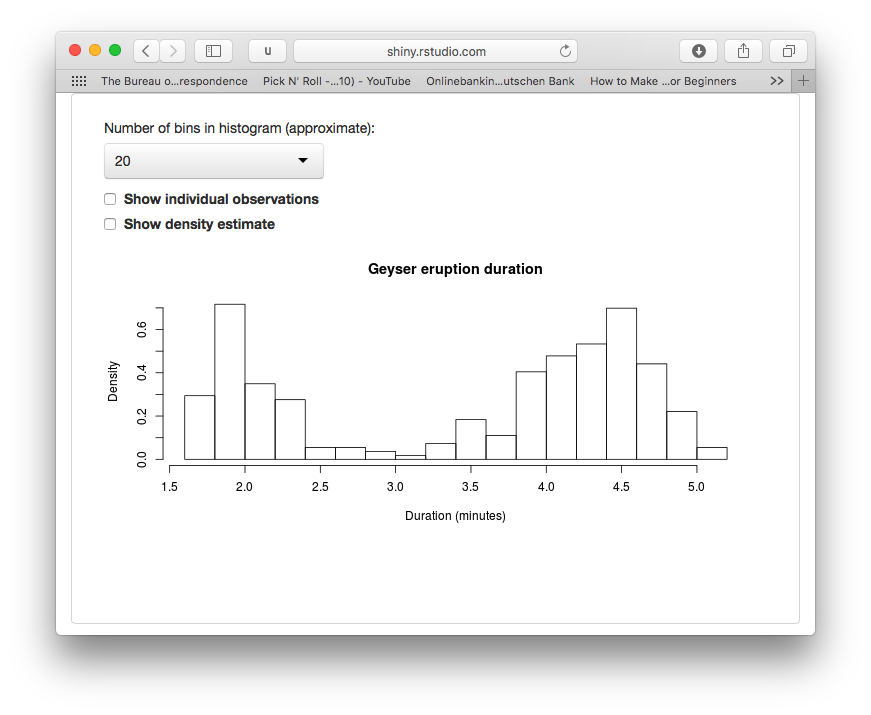
\includegraphics[scale = 0.5, trim = 50 50 50 100]{figures/example_shiny_app.png}
\caption{Screenshot of an example Shiny Application.}
\label{exampleapp}
\end{centering}
\end{figure}

Figure \ref{exampleapp} shows an example Shiny Application, consisting of some user interface (UI) control elements (a select button, and tick boxes) and a graph. The UI is reactive; whenever the user ticks a box or selects a different value in the first box, the graph changes its look. This is built upon reactive functions, which run every time a value inside them changes. The values that are allowed to change are therefore bound to the UI elements.

Shiny Apps consist of two elements: The UI and a ``server" side. The UI includes functions which wrap HTML to build the viewable part of the App, for example buttons and placement of graphs. The server side consists of functions that specify the reactive R functions which create dynamic output displayed on the UI side, and when the functions should be run. Both sides then are able to automatically communicate with each other to create a smooth interactive experience for the user. The code for an example Shiny app is attached below:

\begin{lstlisting}[caption = Example code for a Shiny Application\cite{w2}., label = code:exampleapp]
# Define UI
ui <- bootstrapPage(
  numericInput("n", "Number of obs", 100),
  plotOutput("plot")
)
# Define Server
server <-  function(input, output) {
  output$plot <- renderPlot({ hist(runif(input$n)) })
}
app <- shinyApp(ui, server)
# Run App
runApp(app)
\end{lstlisting}

It is now possible to see in Code-Chunk \ref{code:exampleapp} that both the UI and server elements are R objects, while the server also resembles an R function. \li{runApp()} then opens up the Application.

\subsection{Shiny Gadgets and RStudio Add-Ins}
\label{shinyrstudiochapter}

Shiny Applications are useful for displaying interactive visualisations, but they are made for displaying results to the end user. ``Shiny Gadgets"\footnote{\url{http://shiny.rstudio.com/articles/gadgets.html}}, an extension of the Shiny framework, are supposed to be part of the programming or analysing process. They are built on the same framework that was introduced with Shiny, but serve the purpose of making programming challenges a little easier. For example, a Shiny Gadget could be used to provide a UI for downloading certain data from complex websites. 

``RStudio Add-Ins"\footnote{https://rstudio.github.io/rstudioaddins/} are Shiny Gadgets that are built right into RStudio, an Integrated Developer Environment (IDE) for R. Calling the Shiny Gadget is made easier, as the RStudio user only has to press two buttons. Furthermore, Add-Ins have extended access to RStudio itself via a package called ``rstudioapi". For example, Add-Ins are able to paste a string into the console and can modify the currently opened R script.

The combination of the Shiny framework and RStudio add-ins creates the ideal setting for an Add-In that helps the user parse any data format into R. The Shiny Framework provides interactiveness and the RStudio connection makes it easier to call the Application out of an IDE.

\section{Implementation}

An R-Studio Add-In has to be installed via the R package ecosystem, so GREA is also wrapped up in a package called GREA. Calling the Add-In is done via the main function \li{GREA::GREA()}. Also, there exist a couple of helper functions, which were necessary to reduce redundant R code.
The following functions are implemented:

\begin{itemize}
\item \li{GREA()}
\item \li{GREA_read()}
\item \li{wd_check()}
\item \li{fileChoose()}
\end{itemize}

As stated above, \li{GREA::GREA()} is the function that starts the Add-In. \li{GREA::GREA_read()} is the most important helper function, which converts any filetype into the data.frame R class inside the global environment. For checking if a file is inside the current R working directory, \li{GREA::wd_check()} was written. This function arose from my personal frustration with large filepaths. \li{GREA::fileChoose()} has the same utility as \li{base::file.choose()} (choosing a file interactively), except that it returns \li{NULL} when cancelled.

\subsection{The Main Function: \textrm{GREA()}}
As explained in Chapter \ref{shinyrstudiochapter}, Add-Ins are built on the Shiny Framework. \li{GREA()} is therefore also a wrapper for a Shiny Application. In this section, the general structure of the function will be demonstrated.

\begin{lstlisting}[caption = Structure of the \li{GREA()} function, label = greacode]
GREA <- function() {
  ui <- miniPage(
    # User Interface Functions #
    # ...
  )
  server <- shinyServer(function(input, output, session) {
    # Reactive Server Functions #
    # ...
    observeEvent(input$done, {
      # Functions that paste the code into the console
    })
  })
  # Functions that start the Add-In
  app <- shinyApp(ui = ui, server = server)
  viewer <- dialogViewer(dialogName = "GREA", 
                         height = 350, width = 500)
  runGadget(app, viewer = viewer, stopOnCancel = FALSE)
}
\end{lstlisting}

Code-Chunk \ref{greacode} shows the structure of GREA's main function. Similarly to Shiny Applications, we can see that the \li{ui}(lines 2-5) and \li{server}(lines 6-12) objects are specified first. For creating the \li{ui} object, the \li{miniUI::miniPage()} function from the miniUI package (cite??) is used, which is specifically targeted at small user interfaces in the style of smartphone apps. The \li{server} object, also resembling an R function, consists of reactive functions that are called every time the user interacts with the UI. This includes the selection of a file to be read in on the user's computer, or the adjustment of reading conditions (e.g. a change in the comma seperator in text-delimited files).

Next, both objects are assembled to a new object called \li{app}(line 14). In lines 15 and 16, an object named \li{viewer} is generated via \li{shiny::dialogViewer()}. This step ensures that GREA is started as an integrated window in RStudio with the right height and width. In the end, the function \li{runGadget()}(line 17) is called to start the Add-In. In essence, this function has the same functionality as the \li{shiny::runApp()} function, with the addition of better automatic handling in the event of the user cancelling the app.

The piece of code that sets this Add-In apart from Shiny applications and Shiny Gadgets is resembled by the contents of lines 9-11, a function which is run when the user presses the ``done" button.

\begin{lstlisting}[caption = Contents of reactive function for ``Done"-event, label = doneeventcode]
observeEvent(input$done, {
  # Paste Code into Console
  if (nzchar(fileloc()) && nzchar(input$name_dataset) && !is.null(dataset())) {
    # Get code that was used to read dataset
    expr <- attributes(dataset())$GREAcommand
    # Assemble code
    code <- paste0(input$name_dataset, " <- ", expr)
    # Paste into Console
    rstudioapi::insertText(text = code, id = "#console")
  }
  # ... and then stop the app
  stopApp()
})
\end{lstlisting}

Code-Chunk \ref{doneeventcode} shows the detailed contents of lines 9-11 in Code-Chunk \ref{greacode}. After the user has specified all necessary variables interactively, she/he presses the ``done" button. This triggers the event called \li{input$done}, which leads to the above function being called.

Line 3 checks if three conditions are met: 
\begin{enumerate}
\item A file location is correctly specified.
\item A dataset name is correctly specified.
\item Reading the dataset with the options provided by the user is successful.
\end{enumerate}

These conditions make sure that the user doesn't obtain code for reading a file which will yield an error. If and only if these conditions are met, the code to read the data is assembled (lines 5-7)  and then pasted into the R console (line 9). The procedure to paste the code into the console makes use of the \li{insertText()} function from the ``rstudioapi" package, previously mentioned in Chapter \ref{shinyrstudiochapter}. After this procedure, the user obtains the code to read the specified file and only has to execute the command to attach the new data to R's global environment.

irgendwo muss hier noch rein was alles dazwischen passiert und wo sozusagen die specifications sind vor allem im server

vielleicht implementation vor das andere packen?

\subsection{The File Reading Function: \textrm{GREA\_read()}}
Chapter blabla explained the implementation of the main function, \li{GREA::GREA()}. The core to this function is the function that reads filetypes into R.
Writing this function was the most challenging, as it had to fulfill the following requirements at once:
\begin{enumerate}
\item Read a filetype and convert it to an R object
\item Keep the code after a successful reading 
\item Omit rarely used arguments in the code that should be pasted into the console
\end{enumerate}
\subsection{Helper Functions}
\section{Usage}


\clearpage

\section*{Appendix}
\addcontentsline{toc}{section}{Appendix}

\begin{thebibliography}{59}
\begin{singlespace}

\bibitem{w1}
The Comprehensive R Archive Network. (2016) 'Contributed Packages'. \emph{CRAN}.
Available: \url{https://cran.r-project.org/index.html} 
[Accessed 4 August 2016].

\bibitem{w2}
W. Chang et al (2016).
\emph{shiny: Web Application Framework for R}. R package version 0.13.2.
\url{https://CRAN.R-project.org/package=shiny}

\end{singlespace}
\end{thebibliography}
\end{document}